\documentclass[]{article}
\usepackage{lmodern}
\usepackage{amssymb,amsmath}
\usepackage{ifxetex,ifluatex}
\usepackage{fixltx2e} % provides \textsubscript
\ifnum 0\ifxetex 1\fi\ifluatex 1\fi=0 % if pdftex
  \usepackage[T1]{fontenc}
  \usepackage[utf8]{inputenc}
\else % if luatex or xelatex
  \ifxetex
    \usepackage{mathspec}
  \else
    \usepackage{fontspec}
  \fi
  \defaultfontfeatures{Ligatures=TeX,Scale=MatchLowercase}
\fi
% use upquote if available, for straight quotes in verbatim environments
\IfFileExists{upquote.sty}{\usepackage{upquote}}{}
% use microtype if available
\IfFileExists{microtype.sty}{%
\usepackage{microtype}
\UseMicrotypeSet[protrusion]{basicmath} % disable protrusion for tt fonts
}{}
\usepackage[margin=1in]{geometry}
\usepackage{hyperref}
\hypersetup{unicode=true,
            pdftitle={Effect of Trump's tweets on oil price (732A92)},
            pdfauthor={Pedram Kasebzadeh(pedka102)},
            pdfborder={0 0 0},
            breaklinks=true}
\urlstyle{same}  % don't use monospace font for urls
\usepackage{longtable,booktabs}
\usepackage{graphicx,grffile}
\makeatletter
\def\maxwidth{\ifdim\Gin@nat@width>\linewidth\linewidth\else\Gin@nat@width\fi}
\def\maxheight{\ifdim\Gin@nat@height>\textheight\textheight\else\Gin@nat@height\fi}
\makeatother
% Scale images if necessary, so that they will not overflow the page
% margins by default, and it is still possible to overwrite the defaults
% using explicit options in \includegraphics[width, height, ...]{}
\setkeys{Gin}{width=\maxwidth,height=\maxheight,keepaspectratio}
\IfFileExists{parskip.sty}{%
\usepackage{parskip}
}{% else
\setlength{\parindent}{0pt}
\setlength{\parskip}{6pt plus 2pt minus 1pt}
}
\setlength{\emergencystretch}{3em}  % prevent overfull lines
\providecommand{\tightlist}{%
  \setlength{\itemsep}{0pt}\setlength{\parskip}{0pt}}
\setcounter{secnumdepth}{0}
% Redefines (sub)paragraphs to behave more like sections
\ifx\paragraph\undefined\else
\let\oldparagraph\paragraph
\renewcommand{\paragraph}[1]{\oldparagraph{#1}\mbox{}}
\fi
\ifx\subparagraph\undefined\else
\let\oldsubparagraph\subparagraph
\renewcommand{\subparagraph}[1]{\oldsubparagraph{#1}\mbox{}}
\fi

%%% Use protect on footnotes to avoid problems with footnotes in titles
\let\rmarkdownfootnote\footnote%
\def\footnote{\protect\rmarkdownfootnote}

%%% Change title format to be more compact
\usepackage{titling}

% Create subtitle command for use in maketitle
\providecommand{\subtitle}[1]{
  \posttitle{
    \begin{center}\large#1\end{center}
    }
}

\setlength{\droptitle}{-2em}

  \title{Effect of Trump's tweets on oil price (732A92)}
    \pretitle{\vspace{\droptitle}\centering\huge}
  \posttitle{\par}
    \author{Pedram Kasebzadeh(pedka102)}
    \preauthor{\centering\large\emph}
  \postauthor{\par}
      \predate{\centering\large\emph}
  \postdate{\par}
    \date{2/11/2020}


\begin{document}
\maketitle

\newpage 

\section{Abstract}\label{abstract}

\section{Abstract}\label{abstract-1}

Donald Trump, the current president of the united states, has always
been very active on social media. His explicit words have been on the
top of the news many times. His post on Twitter(tweets) are the subject
of this project. The goal of this project is to study the correlation
between his tweets and the oil price in the international market.

To do so I performed sentiment analysis on a data sets of tweets, and
gave a total point to his tweets per day, and tried to compare them to
the variation of in oil price. I used two different methods of sentiment
analysis (NRC and Bing).

\newpage

\tableofcontents

\newpage

\section{Introduction}\label{introduction}

Number of social media users, more specifically Twitter, have been
dramatically increased over the past decade(Clement
\protect\hyperlink{ref-j_clement_twitter_2019}{2019}). And it plays a
huge role in different aspects of our lives, politics and economics for
instance. It plays a huge role in elections as well. Donald Trump tweets
are the subject of this report, the president of the united states who
tweets very often and is known for his harsh tweets. In the previous US
election, most of his top tweets aside from ``Mexico will pay for the
wall!'' were attacks against other candidates and their supporters,
rather than discussing politics! (Magdy and Darwish
\protect\hyperlink{ref-magdy_trump_2016}{2016})

In this report, I will try to find any possible correlation between
Trump tweets and oil price. The reason I wanted to investigate this is
that his tweets usually have a big impact on Iran's economy. The impact
is so significant that his daily tweets not only would affect Iran's
currency value but also could have an effect on product prices in the
markets in Iran the day after!

Although all of this could be based on the complicated relationship
between Iran and the US or the corruption in Iran's regime, which drives
based on spreading hate against the united states and looks for any
possibility to make a profit out of it. All of this made me curious to
see if his words are as important in the global community and would have
any effect on some fragile variable like oil price.

My approach to doing so was doing sentiment analysis. I used 3 datasets
and 3 methods which I will explain in detail furthermore.

\section{Theory}\label{theory}

Sentiment analysis (also known as opinion mining or emotion AI) refers
to the use of natural language processing, text analysis, computational
linguistics, and biometrics to systematically identify, extract,
quantify, and study affective states and subjective information.
Sentiment analysis is widely applied to the voice of the customer
materials such as reviews and survey responses, online and social media,
and healthcare materials for applications that range from marketing to
customer service to clinical medicine. (wikipedia, n.d.) however, in
this case, I focused on the voice of only 1 person. The idea was to
categorize Trump's tweets.

Sentiment analysis is a strategy to explore whether a gathered content
is in a positive, negative or neutral state, it could be done in
different levels such as Sentence level, Document-level, Aspect level or
user level (International Conference on Automation et al.
\protect\hyperlink{ref-international_conference_on_automation_abstract_2019}{2019}).

Sentiment analysis uses various Natural Language Processing (NLP)
methods and algorithms, 3 main types of algorithms used are: Rule based
(systems that perform sentiment analysis based manually crafted rules),
Automatic(systems that rely on machine learning techniques), And
Hybrid(systems that used a mix of the first two).(``Sentiment Analysis''
\protect\hyperlink{ref-noauthor_sentiment_2020}{2020})

In This project, I decided to focus on doing sentiment analysis over
tweets which could be considered the same as sentence-level sentiment
analysis. I used a Rule based algorithm which uses Lexicons (i.e.~lists
of words and expressions). Then I summed up the point of all the tweets
for each day to get a conclusion of how did his tweets grade overall.

To find any relations between the tweets and oil price I used Pearson
correlation.

\[  \rho_{X,Y}= \frac{\text{cov}(X,Y)}{\sigma_X\sigma_Y}\]

I also used 3 manually created lexicons, the NRC Emotion Lexicon (Saif M
Mohammad and Turney \protect\hyperlink{ref-mohammad_nrc_2013}{2013})
(about 14,000 words), AFINN (Nielsen
\protect\hyperlink{ref-nielsen_new_2011}{2011}) (about 2477 words and
phrases), and the Bing Liu Lexicon(Kohavi and Computing Machinery
\protect\hyperlink{ref-kohavi_kdd-2004_2004}{2004}) (about 6,800 words).

\section{Data}\label{data}

Collecting data for this project was a bit challenging. First, I used
twitter APIs to collect data, however, the limitations made it not the
best approach. So, I found a huge data set of tweets from many US
politicians with 1.6 GB size and extracted Trump tweets. That left me
with 7300 tweets from Trump in the period of 16th of July 2015 to the
first of November 2016. which was not the best dataset since Trump
became president as of January 20, 2017. I assumed there is a huge
difference between a president tweet and a businessman tweet, which made
this whole dataset useless.

My data sets are from a website (archive, n.d.), this is a website
mainly focused on Trump's tweets and gives a variety of options on how
to filter tweets before extraction. I extracted 2 data sets from this
website.

The first one was filtered with words like ``oil'', ``Opec'', ``Iraq'',
``Saudi'', ``Gulf'' and ``Iran'' in the tweets, and just extracting
tweets with such words. I tried to find the most related words to the
matter by going through some of his tweets and my idea of the concept.
The filtered data set has 2317 tweets in it. One critical detail about
this data set was that it was not filtered by date, so there were some
dates without any tweets, which is a bit different from the usual
Trump's activity, that being said the dataset was dated between May 2009
and February 2020.

The second dataset was a data set of all of the tweets provided on the
website, which was 46040 tweets from April 2009 to February 2020.

\begin{figure}
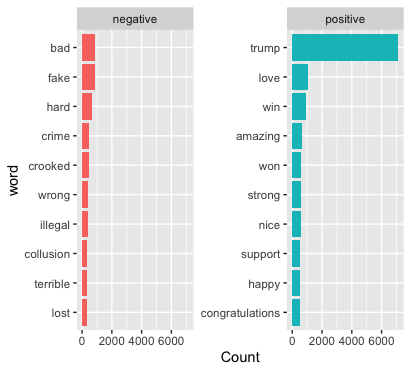
\includegraphics[width=35cm,
  height=10cm,
  keepaspectratio]{Count}
\centering 
\caption{Top 10 Negative and Positive words}\label{Figure1}
\end{figure}

Figure1 shows a short illustration of the 10 most used words
distribution in 2 categories, `positive' and `negative'. one interesting
observation was how often Trump uses his name in his tweets and that
Bing lexicon would categorize it as a Positive word! I did think about
removing it from the tweets, however, since the goal is to find
correlations a constant plus 1 in the scores would have no effect.

The Third dataset I needed was the oil price which is documented and was
fairly easy to collect. (Thomson, n.d.) This dataset consists of daily
oil prices for May 20th, 1987 until February 24th, 2020. Of course, I
did not use the whole dataset in my case, since there was no twitter
before 2006 and Trumps activity started 3 years after that on, May 2009,
so a noticeable amount of the data set was useless which I removed by
merging this data set with the other 2 in separate steps.

\begin{figure}
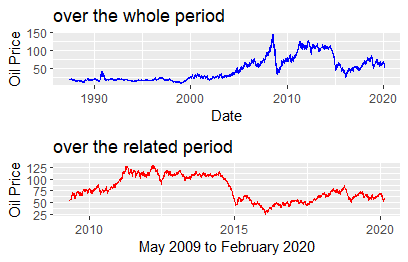
\includegraphics{oilprice}
\centering 
\caption{Oil Price over different timelines}\label{Figure2}
\end{figure}

That being said, Figure 2 shows two plots, one of the oil prices over
the whole time and the second one shows oil prices since 2009(Trump's
joining date).

For evaluation purposes, I also used movie reviews dataset from text
mining lab 3 (``Product Reviews,'' n.d.), as I needed a labeled dataset.

\subsection{preprocessing}\label{preprocessing}

To do this project, after collecting the data the most essential part
was data cleaning. Data cleaning refers to identifying incomplete,
duplicate, incorrect, inaccurate or irrelevant parts of the data and
then replacing, modifying, or deleting the dirty or coarse
data.(International Conference on Automation et al.
\protect\hyperlink{ref-international_conference_on_automation_abstract_2019}{2019})
to do so I had to use different libraries and multiple functions.

In my survey of related work, I came across a sarcasm detection system
that could be helpful on the data cleaning phase, However, I did not use
it, as I was considered it might not be reliable on detecting sarcasm
over Trump's tweets as even I as a human sometimes find it challenging.

\section{Method}\label{method}

My method consists of 3 parts:

\begin{enumerate}
\def\labelenumi{\arabic{enumi}.}
\tightlist
\item
  Find reliable list of words with strongly positive or negative
  sentiment. (lexicons)
\item
  Count the number of positive and negative words in each tweet.\\
\item
  Summing up the scores based on number of positive and negative words.
\end{enumerate}

After cleaning the data, As I had 3 different methods to get the
sentiment with, and 2 data sets, I created a function with all the
necessary sentiment functions (such as tokenization) inside it, so it
was more convenient to work with. Instead of running 6 functions I ran
1, twice. For creating the functions and performing sentiment analysis,
I chose R language, it has a lot of text mining packages and is a great
tool to manipulate huge datasets.(Tatman, n.d.)

\subsection{Evaluation}\label{evaluation}

Since I could not find any reliable labeled dataset for Trump's tweets,
which is needed for classification with Naïve Bayes, Logistic Regression
or Support Vector Machines, I decided to test out my functions on the
dataset we already used in our text mining course(732A92) (``Product
Reviews,'' n.d.). Which is a labeled dataset of movie reviews with two
possible levels ``positive'' and ``negative''.

For evaluation I compared the accuracy I had using my function with the
Sentiment Analysis function by Stefan Feuerriegel and Nicolas
Proellochs(Feuerriegel and Proellochs
\protect\hyperlink{ref-feuerriegel_sentimentanalysis_2019}{2019}).

For the accuracy to make sense I had to transform ``Positive'' and
``negative'' of the data set to +1 and -1 values accordingly.

I used my function and Stefan's function both on the labeled dataset
from the course to see how accurate they can predict the sentiment of a
movie review. Based on the obtained results my function was more
accurate with any of the 3 lexicons used.

\section{Result}\label{result}

In this section, you can see the result of my work, presented in graphs
and tables.

\begin{figure}
\includegraphics[width=15cm,
  height=10cm,
  keepaspectratio]{filtered}
\centering 
\caption{Scores for filtered data}\label{Figure3}
\end{figure}

In Figure3 we have the results for 3 different methods over-filtered
data, However, it might be a bit messy at first glance, we can see
different scaling for different methods (for instance AFINN has an
indicator for sentiment between -5 and 5). we also have scaled oil
prices just to have a resemblance to the big picture.

\begin{figure}
\includegraphics[width=15cm,
  height=10cm,
  keepaspectratio]{fulldata}
\centering
\caption{Scores for the whole dataset}\label{Figure4}
\end{figure}

Figure4 reveals results for 3 different methods over the second dataset
(the big non-filtered one). Below you can see a table of the correlation
and p-values in the filtered dataset for different methods.

\begin{longtable}[]{@{}lcr@{}}
\toprule
Method & Correlation & P-Value\tabularnewline
\midrule
\endhead
NRC & -0.07901497 & 0.003523\tabularnewline
Bing & -0.01280621 & 0.6368\tabularnewline
Afinn & -0.0554452 & 0.04076\tabularnewline
\bottomrule
\end{longtable}

Below is a table of p-values and correlations of the non-filtered
dataset for different methods.

\begin{longtable}[]{@{}lcr@{}}
\toprule
Method & Correlation & P-Value\tabularnewline
\midrule
\endhead
NRC & 0.07824593 & 9.487e-06\tabularnewline
Bing & 0.04989503 & 0.004782\tabularnewline
Afinn & 0.06836199 & 0.0001099\tabularnewline
\bottomrule
\end{longtable}

\newpage 

\subsection{Evaluation results}\label{evaluation-results}

After comparing my method with Stefan function, I obtained higher
accuracy on predicting movies reviews sentiment. Below you can see the
result in a table.

\begin{longtable}[]{@{}lccr@{}}
\toprule
NRC & Bing & Afinn & Stefan\tabularnewline
\midrule
\endhead
\%63 & \%75 & \%70 & \%57\tabularnewline
\bottomrule
\end{longtable}

\section{Discussion}\label{discussion}

Figure4 reveals some interesting facts! As we can see in this plot
scores are going too high or too low, considering the fundamentals of
each method's score, the reason for this could be a lot of same
sentiment tweets in one day. For instance, over 20 positive tweets in
one day and maybe 30 negative tweets the day after. There might be very
interesting psychological data to be discovered here.

On the filtered dataset we have an insignificant negative correlation
which(assuming critical p-value is 0.05) indicates that when Trump's
tweets related to oil are negative it could have a slight increase in
the oil price, However in the non-filtered data set which is a
collection of all of his tweets we have a positive correlation which
means when he tweets something positive price would go up and when he
tweets something negative price goes down. So we can that filtered data
set is somewhat closer to our assumption however both of them are still
very weak correlations.

On the evaluation set, I noticed I have got a higher accuracy for Bing
and AFINN, compared to NRC even though they have smaller word database,
which means using the bigger lexicon will not always give us the best
result.

Several possibilities of improving the performance of the models
exist.Maybe using some groups of features would find a better
understanding of what Trump says and ends up on better results, as we
can see in (Saif M. Mohammad, Kiritchenko, and Zhu
\protect\hyperlink{ref-mohammad_nrc-canada_2013}{2013}), doing so,
resulted in great accuracy on sentiment analysis.

Also maybe scaling lexicon scores and merging the results is something
to think about, I believe that is one thing missing from my approach,
The reason I did not implement it was that I could not think of an
efficient and reasonable way to merge these numbers, to be more clear
AFINN has a range of +5 and -5 however Bing does not have such
limitation, Hence I am not sure how I should compare a 5 resulted with
AFINN and a -6 given by Bing. Such concerns resulted in presenting each
method separately instead of merging the results.

\section{Conclusion}\label{conclusion}

There was not any noticeable correlation between Trump's tweets and oil
price fluctuations, so that means my assumption was not correct under
these circumstances, which means. Oil price is not affected by what only
1 man has to tweet, even if that man is the president of the united
states of America.

Another good approach for future analysis could be using a dataset based
on a specific time (e.g.~when there are a lot of rumors about a war in
the middle east) rather than focusing on one person.

One thing I'm curious about is the accuracy of used and available
methods for doing sentiment analysis over Trump's tweets and speeches as
he is usually using very unusual structures of language and has a unique
choice of words. A manually labeled set of data of his tweets is the one
way, that comes to mind, to obtain any reliable accuracy of our method
functioning.

\newpage

\section*{References}\label{references}
\addcontentsline{toc}{section}{References}

\hypertarget{refs}{}
\hypertarget{ref-trump_twitter_archive_trump_nodate}{}
archive, Trump twitter. n.d. ``Trump Twitter Archive.''
\url{http://www.trumptwitterarchive.com/}.

\hypertarget{ref-j_clement_twitter_2019}{}
Clement, J. 2019. ``Twitter Useres.'' August 14.
\url{https://www.statista.com/statistics/282087/number-of-monthly-active-twitter-users/}.

\hypertarget{ref-feuerriegel_sentimentanalysis_2019}{}
Feuerriegel, Stefan, and Nicolas Proellochs. 2019. ``SentimentAnalysis
Vignette.'' March 26.
\url{https://cran.r-project.org/web/packages/SentimentAnalysis/vignettes/SentimentAnalysis.html}.

\hypertarget{ref-international_conference_on_automation_abstract_2019}{}
International Conference on Automation, Computational and Technology
Management, Amity University, Institute of Electrical and Electronics
Engineers, United Kingdom and Republic of Ireland Section, and Institute
of Electrical and Electronics Engineers. 2019. \emph{Abstract
Proceedings of International Conference on Automation, Computational and
Technology Management (ICACTM-2019): 24th - 25th April 2019}.
\url{https://ieeexplore.ieee.org/servlet/opac?punumber=8766340}.

\hypertarget{ref-kohavi_kdd-2004_2004}{}
Kohavi, Ron, and Association for Computing Machinery, eds. 2004.
\emph{KDD-2004: Proceedings of the Tenth ACM SIGKDD International
Conference on Knowledge Discovery and Data Mining: August 22-25, 2004,
Seattle, Washington, USA}. New York: ACM Press.

\hypertarget{ref-magdy_trump_2016}{}
Magdy, Walid, and Kareem Darwish. 2016. ``Trump Vs. Hillary Analyzing
Viral Tweets During US Presidential Elections 2016.''
\emph{arXiv:1610.01655 {[}Cs{]}}, November.
\url{http://arxiv.org/abs/1610.01655}.

\hypertarget{ref-mohammad_nrc_2013}{}
Mohammad, Saif M, and Peter D Turney. 2013. ``Nrc Emotion Lexicon.''
\emph{National Research Council, Canada}.

\hypertarget{ref-mohammad_nrc-canada_2013}{}
Mohammad, Saif M., Svetlana Kiritchenko, and Xiaodan Zhu. 2013.
``NRC-Canada: Building the State-of-the-Art in Sentiment Analysis of
Tweets.'' \emph{arXiv:1308.6242 {[}Cs{]}}, August.
\url{http://arxiv.org/abs/1308.6242}.

\hypertarget{ref-nielsen_new_2011}{}
Nielsen, Finn Årup. 2011. ``A New ANEW: Evaluation of a Word List for
Sentiment Analysis in Microblogs.'' \emph{arXiv:1103.2903 {[}Cs{]}},
March. \url{http://arxiv.org/abs/1103.2903}.

\hypertarget{ref-noauthor_product_nodate}{}
``Product Reviews.'' n.d.
\url{https://www.ida.liu.se/~732A92/commons/reviews.json.bz2}.

\hypertarget{ref-noauthor_sentiment_2020}{}
``Sentiment Analysis.'' 2020. January.
\url{https://monkeylearn.com/sentiment-analysis/}.

\hypertarget{ref-tatman_sentiment_nodate}{}
Tatman, Rachael. n.d. ``Sentiment Analysis in R.''
\url{https://www.kaggle.com/rtatman/tutorial-sentiment-analysis-in-r}.

\hypertarget{ref-thomson_europe_nodate}{}
Thomson, Reuters. n.d. ``Europe Brent Spot Price FOB Dollars Per
Barrel.'' \url{https://www.eia.gov/dnav/pet/hist/RBRTED.htm}.

\hypertarget{ref-wikipedia_sentiment_nodate}{}
wikipedia. n.d. ``Sentiment Analysis.''
\url{https://en.wikipedia.org/wiki/Sentiment_analysis\#References}.


\end{document}
